% $Id: introduction.tex 87303 2016-02-08 13:44:29Z lafferty $

\subsection{Analysis strategy}
\label{subsec:strategy}

Decays of the \KS in LHCb are characterized by decay vertices separated from the interaction point\footnote{The \KS at LHC typically decays after traversing tens of centimeters to even several meters.}, 
and with tracks having an average transverse momentum significantly lower than those from $b$ and $c$ decays.
The transverse momentum range is similar to typical tracks generated in the proton-proton collision and hence has almost no discriminating power. 

Muon candidates are combined into $\mu^+\mu^-$ pairs. Then a $\pi^0$ can be added to the dimuon pair to make a fully reconstructed
\KS decay. However, since the reconstruction efficiency of the $\pi^0$ is limited, events in which no $\pi^0$
is found are also considered, based only on the dimuon information. This leads to two independent analyses: one for the
events in which all decay products are considered (hereafter FULL) and one in which only the dimuon pair is used
(hereafter PARTIAL). 
The reconstructed candidates are then passed through a selection algorithm followed by a {\it Boosted Decision Tree} (BDT) classification,
to reduce the high level of background.


The properties of the \Kspizmm decays are studied using simulated samples with a differential decay rate modeled according to Ref.~\cite{Gino}.
The corresponding $\mumu$ mass distribution, $m_{\mumu}$, as well as the dependence of the (cosine of the) dimuon helicity 
angle, $\cos\theta_{\mu}$ (see the angle definitions in \figref{fig:angles}), on $m_{\mumu}$ are shown in \figref{fig:EviltGen}.

 \begin{figure}[htb!]
 \begin{center}
  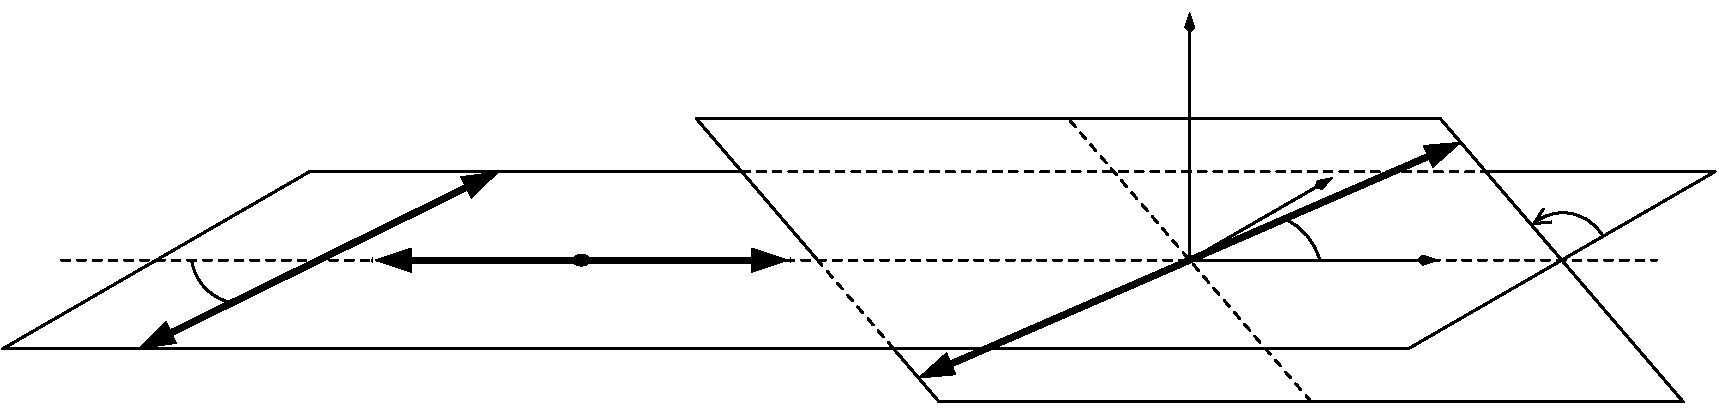
\includegraphics[scale=0.4]{figs/Kspi0MuMu/helAngles.pdf}
  \put(-27,40){${\phi_{\mu}}$}
  \put(-70,35){${\theta_{\mu}}$}
  \put(-308,21){${\phi_{\pi}}$}
  \put(-64,54){$\mu^{-}$}
  \put(-142,5){$\mu^{+}$}
  \put(-272,34){$\pi^0$}
  \put(-225,36){$\KS$}
  \put(-275,18){$\gamma$}
  \put(-250,34){$\gamma$}
  \caption{Definition of the helicity angles in the \KS\ rest frame. \label{fig:angles}}
  \end{center}

 \end{figure}

\begin{figure} [htb!]
\begin{center}
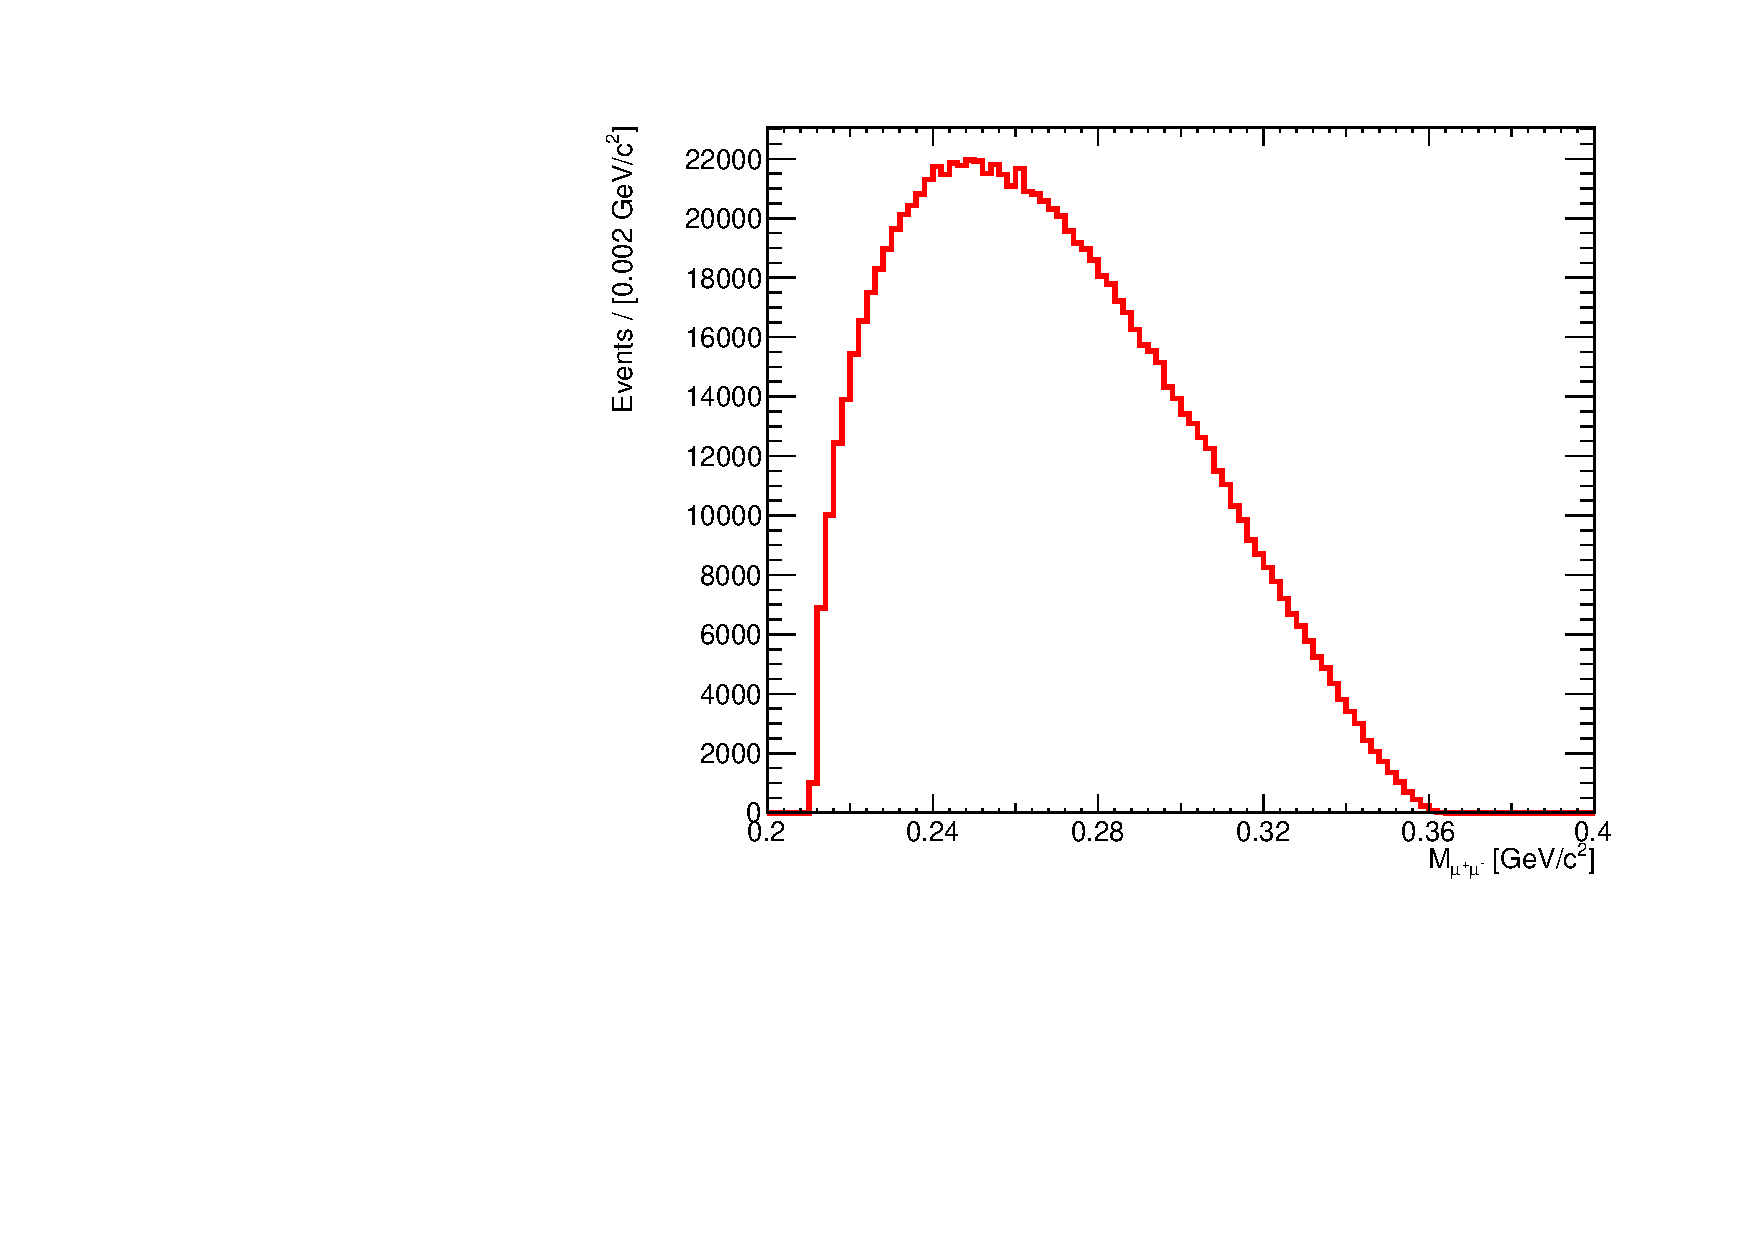
\includegraphics[scale=0.35]{figs/Kspi0MuMu/M_mumu.pdf}
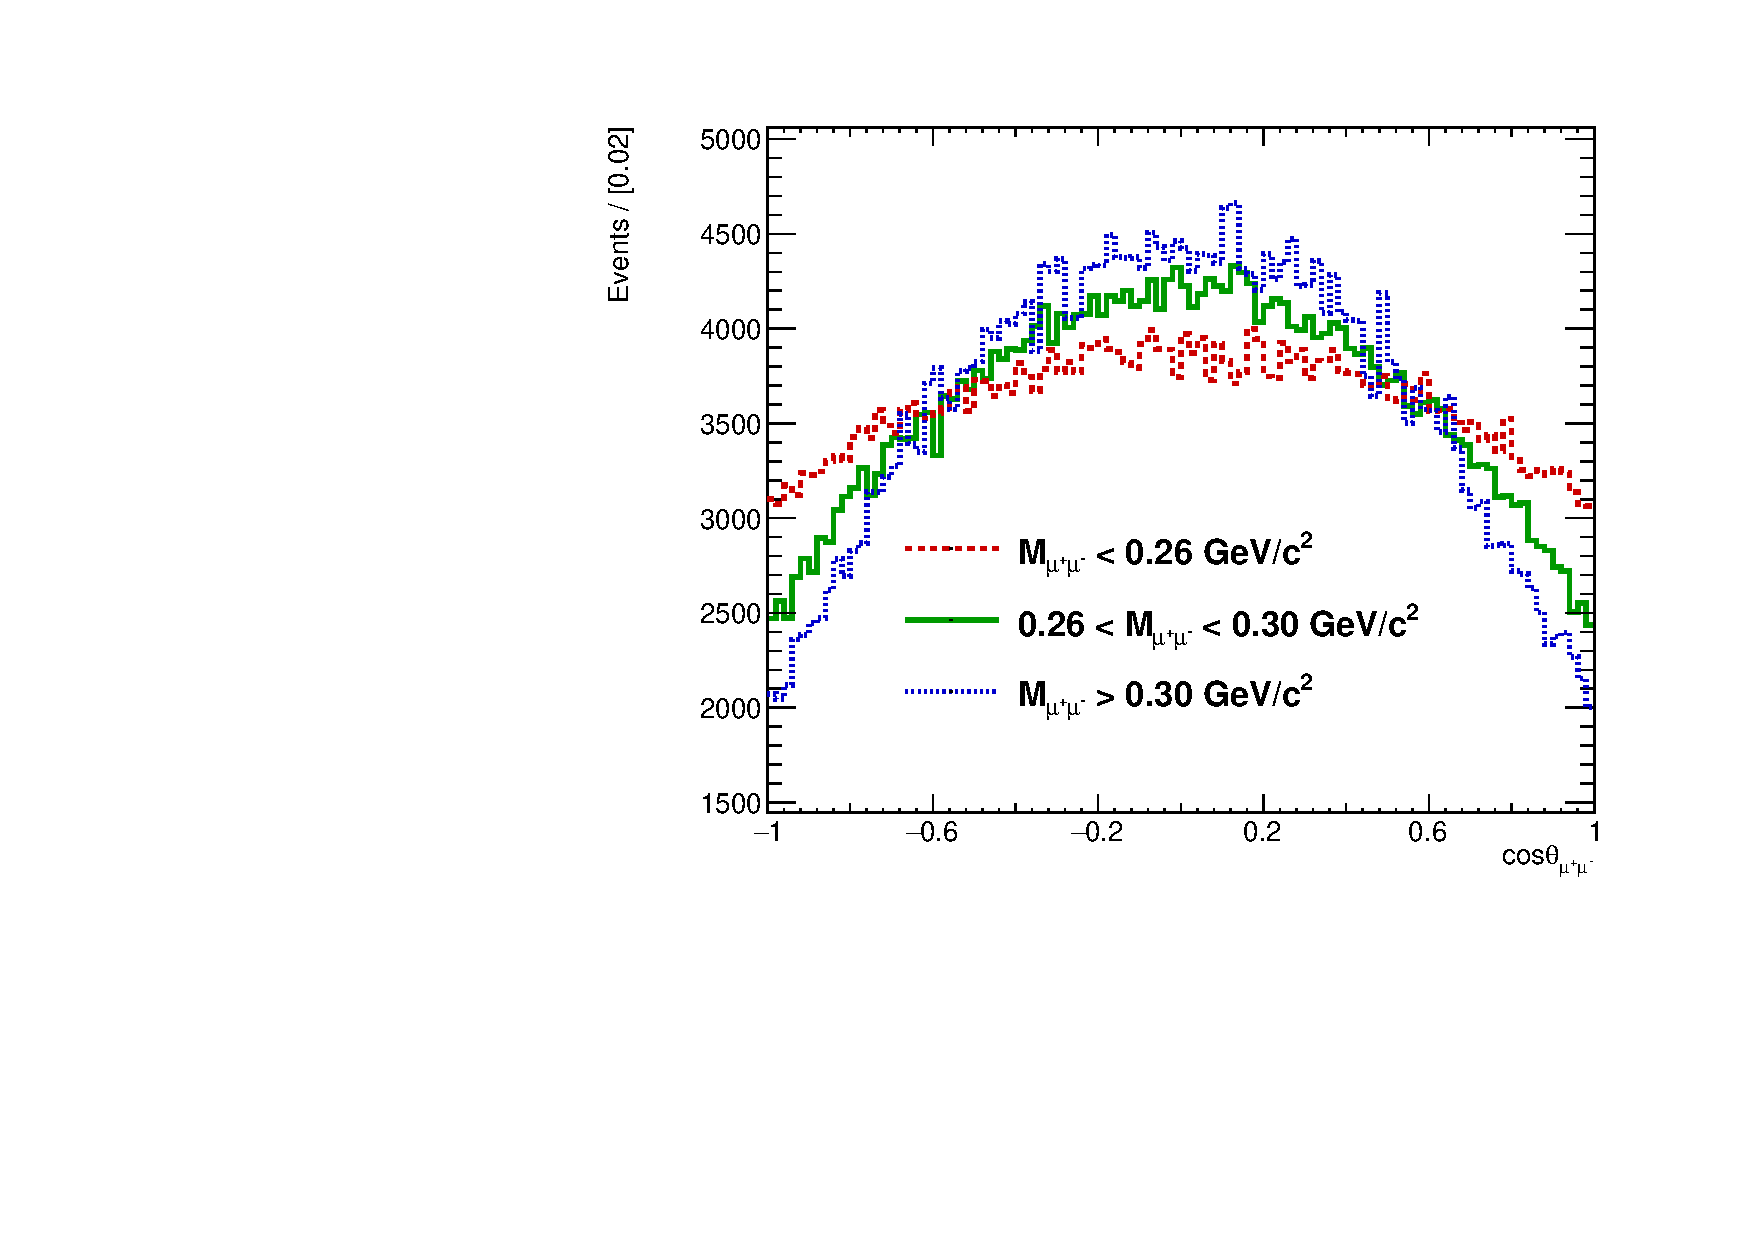
\includegraphics[scale=0.35]{figs/Kspi0MuMu/Hel_mumu.pdf}
\caption{$m_{\mu\mu}$ distribution (left), and the dimuon helicity angle depending on $m_{\mu\mu}$ (right). \label{fig:EviltGen}}
\end{center}
\end{figure}


The BDT is trained with simulated signal events and combinatorial background events from the existing LHCb data.
Since the main goal of this study is to evaluate the sensitivity for the LHCb upgrade, where the
trigger efficiency is expected to be very high, trigger unbiased data samples are preferred.
Therefore, the events are obtained from the {\it Trigger Independent of Signal} (TIS) ~\cite{TISTOS} category of the LHCb trigger. 
This means that the tracks and clusters of the reconstructed candidate are not needed to fire the trigger at any level, because
another object in the underlying event already fired it.
This ensures an almost trigger unbiased data set, while still providing a sample much larger than random selection triggers. 

%The expected signal yield is obtained assuming the NA48 central value for \BRof\Kspizmm, the observed \Kspipi yield from data and
%the efficiency ratio \textcolor{red}{$\frac{\epsilon_{\KsPzMuMu}}{\epsilon_{\PKzS\to\Pgpp\Pgpm}}$} obtained in simulation (See \eqref{eq:normalization}). 

The expected signal yield is obtained assuming the NA48 central value for \BRof\Kspizmm, normalizing the signal yield with respect to \Kspipi as 
\begin{equation}
      \frac{N(\KsPzMuMu)}{N(\PKzS\to\Pgpp\Pgpm)} = 
      \frac{{\cal B}(\KsPzMuMu){\epsilon_{\KsPzMuMu}}}
      {{\cal B}(\PKzS\to\Pgpp\Pgpm){\epsilon_{\PKzS\to\Pgpp\Pgpm}}},
\label{eq:normalization}
\end{equation}
where the observed \Kspipi yield is extracted from data and the efficiency ratio, $\frac{\epsilon_{\KsPzMuMu}}{\epsilon_{\PKzS\to\Pgpp\Pgpm}}$, is obtained from simulation.

The \BRof\Kspizmm sensitivity is measured in a pseudo-experiment study. First, the signal and background yields are extrapolated
for a desired expected luminosity and trigger efficiency, then pseudo-experiments are generated according to those yields. 
The \BRof\Kspizmm uncertainty is obtained from a fit to the \KS mass distribution of the pseudo-experiments, using the signal and background
models obtained from MC and the fit to the available LHCb data, respectively. The mass fit range is $[420,580] \mevcc$.
 


